\chapter{范畴语义}
\section{依值类型的范畴语义}
我们在 \ref{beginning:stlc:canonicity}~节中已经看到代换
的概念是将类型论的语义组织成范畴语言的重要工具. 然而对于
依值类型来说, 代换的陪域与依值函数一样, 取决于自变量的值.
因此这已经无法用范畴中态射直接表达了. 不过, 这个问题早就被
拓扑学家解决过一次了: 对于纤维丛 \(p : E \to B\)
来说, 我们不直接把截面定义为一些依值函数, 而是定义为
\(p\) 的右逆. 换句话说, 我们认为截面是陪域为全空间
的函数 \(s : B \to E\), 而约束 \(p \circ s = \cons{id}\)
保证了 \(s\) 将底空间的每个点射到这个点对应的纤维上.
(TODO: 是否需要科普纤维的概念)

按照这个思路, 我们就能在范畴语言中表述依值类型. 如
\(x{:}A \vdash B(x)\,\text{type}\) 就可以表达为
一个态射 \(p : B \to A\). 对应的一族元素
\(x{:}A \vdash f(x) : B(x)\) 则是满足 \(p \circ s = \cons{id}\)
的态射 \(s\). 将这个想法完善化, 得到的就是依值类型的
范畴语义.

注意以下我们会从语法出发, 试图考察语法中的结构应该对应
范畴语言中的什么. 因此很多时候我们会直接拿语法用在范畴
中, 但是注意这只是为了提供直观看法. 在成品的范畴语义
定义中不会有这些用法.

\subsection{伴随三函子}\berry{2}
为了简化问题, 我们先只考虑一个变量的情况.
如果我们有态射 \(p : B \to A\) 表示类型
\(x{:}A \vdash B\,\text{type}\), 那么
它的\(\Sigma\)-类型很好表达, 就是 \(B \to 1\),
其中 \(1\) 是终对象 (回忆终对象在类型论中对应空语境).
如果我有一个 \(A\) 类型的元素 \(a : 1 \to A\),
那么我希望表达将 \(B\) 的变量 \(x\) 代换掉, 得到的
\(B[x/a]\) 类型. 这正是一个拉回
\[\begin{tikzcd}
  B[x/a] & B \\
  1 & A
  \arrow["a", from=2-1, to=2-2]
  \arrow["p", from=1-2, to=2-2]
  \arrow[from=1-1, to=2-1]
  \arrow[from=1-1, to=1-2]
  \arrow["\lrcorner"{anchor=center, pos=0.125}, draw=none, from=1-1, to=2-2]
\end{tikzcd}\]
在集合范畴中, 这就是原像集合 \(p^{-1}\{a\}\). 而对于
\(\Pi\)-类型而言, 在集合范畴中这定义为 \(p\) 的右逆
构成的集合, 是函数集 \(A \to B\) 的子集. 因此在范畴语言中,
我们先从函数对象 \(B^A\) 出发, 试图描述 “\(p\) 的右逆” 这个条件.

首先我们可以描述复合, 即 \(p^A : B^A \to A^A\). 其次
我们希望取出恒等态射, 即 \(\cons{id}:A \to A\) 对应的
\(1 \to A^A\), 这是函数对象泛性质的直接应用. 接下来取
拉回就得到所需的截面对象.
\[\begin{tikzcd}
  {\Pi p} & {B^A} \\
  1 & {A^A}
  \arrow["{p^A}", from=1-2, to=2-2]
  \arrow[from=2-1, to=2-2]
  \arrow[from=1-1, to=2-1]
  \arrow[from=1-1, to=1-2]
  \arrow["\lrcorner"{anchor=center, pos=0.125}, draw=none, from=1-1, to=2-2]
\end{tikzcd}\]
为了强调这是依值函数的范畴写法, 我们将其写成 \(\Pi p\).
回忆在集合范畴中, 两个函数 \(f,g\) 的拉回就是集合
\(\{(x,y) \mid f(x) = g(y)\}\). 代入\(\Pi p\), 
由于 \(1\) 只有一个元素, 定义可以简化为
\[\Pi p = \{ s \in B^A \mid p^A(s) = \cons{id}\}.\]
而回忆 \(p^A : B^A \to A^A\) 在集合范畴的定义就是
\(p^A(s) = p \circ s\). 因此 \(\Pi p\) 在集合范畴
中确实对应截面的集合.

类似 \(\Pi p\), 我们记 \(p : B \to A\) 的定义域为 \(\Sigma p = B\).

以上解决了在没有其他变量时, \(\Sigma\)-类型、代换、\(\Pi\)-类型
如何表述的问题. 那么在有其他变量时怎么办呢? 由于我们使用
\(1\) 表示空语境, 自然的推广就是把 \(1\) 改成一般的对象.
下面把它展开, 看看这个推广正不正确.

考虑依值类型 \(\Gamma, x{:}A \vdash B\,\text{type}\),
其中 \(B\) 包含变量 \(x\), 以及所有 \(\Gamma\) 中的变量.
由于此时必须有 \(\Gamma \vdash A\,\text{type}\), 我们
首先有一个态射 \(p_A : A \to \Gamma\). (在前面简单情况中,
\(\Gamma\) 是空语境, 因此 \(p_A : A \to 1\) 是指向终对象
的唯一态射.) 接下来, 依值类型 \(B\) 就被解释为态射
\(p_B : B \to A\). 这么看, 一串语境
\(x_1{:}A_1, \dots, x_n{:}A_n\) 就被解释为一串
态射 \(A_n \to A_{n-1} \to \dots \to A_1 \to 1\).
如图, \(A_1 \to 1\) 是平凡的, 而 \(A_2 \to A_1\)
在 \(A_1\) 的十个元素上各有一条纤维 (也就是图中的十块
竖着的长条形区域), 其中画出了最后一条纤维中的元素.
而 \(A_3\) 则是纤维化的纤维化, 四个颜色的区域分别是 \(A_2\) 四个点上的纤维.
\begin{center}
\begin{tikzpicture}
\def\curcircle{ plot[smooth cycle, tension=1.5] coordinates
  {(-4,0) (-3,1.1) (-2,0) (-3.1,-1.1)}}
\begin{scope}\clip\curcircle;
  \begin{scope}
    \clip (-2.2,-1.5) .. controls
      (-2.28, -0.5) and (-2.2,0.5)
      .. (-2.1, 1.5) -- (0,2) -- (0,-2) -- cycle;
    \foreach \yL/\yR/\yLl/\yRl/\color in
      { 2/0.4/4/4/cyan,
        1/0/2/0.4/green,
        0/-0.3/1/0/yellow,
        -4/-4/0/-0.3/pink} {
      \fill[color={\color}] (-4, \yL) to[bend right] (-2, \yR)
        -- (-2, \yRl) to[bend left] (-4, \yLl) -- (-4, \yL);
    }
  \end{scope}
  \draw[gray, thin] (-4, 2) edge[bend right] (-2, 0.4);
  \draw[gray, thin] (-4, 1) edge[bend right] (-2, 0);
  \draw[gray, thin] (-4, 0) edge[bend right] (-2, -0.3);
  \foreach \offset in {0.2,0.4,...,1.8} {
    \draw[thin] ({-4+\offset},-1.5) .. controls
      ({-3.9+\offset*0.9},-0.5) and ({-4+\offset},0.5)
      .. ({-3.9+\offset}, 1.5);
  }
\end{scope} \draw\curcircle;

\node at (-3,-1.5) {\(A_3\)};

\node at (-1,0) {\(\xrightarrow{p_{A_3}}\)};
\def\curcircle{ plot[smooth cycle, tension=1.5] coordinates
  {(0,0) (1,1) (2,0) (1.3,-0.9)}}
\begin{scope}\clip\curcircle;
  \foreach \offset in {0.2,0.4,...,1.8} {
    \draw[gray, thin] ({-0.1+\offset*1.05},-1.5) .. controls
      ({0.1+\offset},-0.5) and ({\offset*1.1},0.5)
      .. ({\offset}, 1.5);
  }
  \fill[blue] (1.96, -0.25) circle (0.04);
  \fill[teal] (1.97, -0.4) circle (0.04);
  \fill[brown] (1.965, -0.55) circle (0.04);
  \fill[purple] (1.95, -0.7) circle (0.04);
\end{scope} \draw\curcircle;
\node at (1,-1.5) {\(A_2\)};

\node at (3,0) {\(\xrightarrow{p_{A_2}}\)};
\def\curcircle{ plot[smooth cycle, tension=1.5] coordinates
  {(4,0) (5.3,0.4) (6,0) (5,-0.3)}}
\draw\curcircle;
\foreach \offset in {0.2,0.4,...,2} {
  \fill ({4+\offset*0.9}, {-\offset*0.1+\offset*\offset*0.1}) circle (0.04);
}
\node at (5,-1.5) {\(A_1\)};

\node at (7.3,0) {\(\xrightarrow{p_{A_1}}\)};
\filldraw (9,0) circle (0.14);
\node at (9,-1.5) {\(1\)};
\end{tikzpicture}
\end{center}
\(\Sigma\)-类型 \(\Gamma \vdash \sum_{x:A}B\)
就对应复合 \(p_A \circ p_B : B \to \Gamma\).
注意这里这个类型仍然保留了 \(\Gamma\) 中的变量. 请读者验证
在集合范畴中这给出的态射确实正确. 从图中看, 从 \(p_{A_3}\)
到 \(p_{A_2} \circ p_{A_3}\), 相当于纵向合并了
\(A_3\) 中的纤维.

给定一个 \(A\) 的元素
\(\Gamma \vdash a : A\), 在范畴论中也即 \(p_A\) 的截面
\(a : \Gamma \to A\). 如果希望代换得到 \(B[x/a]\),
那么也是取拉回:
\[\begin{tikzcd}
  {B[x/a]} & B \\
  \Gamma & A
  \arrow["a", shift left=1, from=2-1, to=2-2]
  \arrow["{p_A}", shift left=1, color={rgb,255:red,128;green,128;blue,128}, from=2-2, to=2-1]
  \arrow["{p_B}", from=1-2, to=2-2]
  \arrow[shift right=1, from=1-1, to=2-1]
  \arrow[shift left=1, from=1-1, to=1-2]
  \arrow["\lrcorner"{anchor=center, pos=0.125}, draw=none, from=1-1, to=2-2]
\end{tikzcd}\]
最后 \(\Pi\)-类型则较为复杂了, 我们希望可以在 \(\Gamma\)
的每个纤维上做类似上文的函数对象拉回的构造. 可以直接试图
从集合范畴中的直觉出发推广, 但是得到的定义会极度繁琐. 我们
已经有了足够的例子, 可以先介绍一个范畴工具.

\begin{definition}
给定范畴 \(\mathcal C\) 中的对象 \(A\),
定义\textbf{俯范畴}(overcategory或slice category)
\(\mathcal C/A\) 的对象为所有形如
\(B \xrightarrow{f} A\) 的态射. 两个对象
\(B \xrightarrow f A\) 与 \(C \xrightarrow g A\)
之间的态射为使得 \(g \circ h = f\) 成立的 \(h\) 的集合.
\end{definition}
这里的 “局部” 指的就是在俯范畴中的构造. 可以在
集合范畴的俯范畴中获取一些直觉: 每个箭头
\(f : B \to A\) 实际上把 \(B\) 拆分成了许多子集
\(B_x = f^{-1}\{x\}\). 而俯范畴 \(\textsf{Set}/A\)
中的所有构造实际上都是这些子集上逐点的构造. 比如
\(B \to A\) 与 \(C \to A\) 在俯范畴中的乘积
\(D \to A\), 满足 \(D_x = B_x \times C_x\).
因此这也称为\textbf{纤维积}, 因为这恰好是每个 \(x\)
的原像 (即 \(x\) 上的\emph{纤维}) 乘起来. 在原范畴
中, 这就是拉回. 在拓扑空间的范畴中这也是类似的, 只不过
纤维之间还自动带有了拓扑信息.

俯范畴的定义中将原来的态射当作新范畴的对象, 容易混淆. 读者
可以思考一道习题确保理解了这个定义.
\begin{lemma}\label{category:sliceslice}
给定态射 \(f : B \to A\), 俯范畴的俯范畴
\(\mathcal C/A/f\) 同构于 \(\mathcal C/B\).
\end{lemma}

利用俯范畴可以更方便地组织已有的表述. 给定态射
\(f : A \to B\), \(\Sigma\) 类型对应着与其直接复合,
这导出了函子 \(\Sigma_f : \mathcal C/A \to \mathcal C/B\).
代换操作对应拉回, 这给出函子
\(f^* : \mathcal C/B \to \mathcal C/A\).
范畴论中, 一旦出现方向相反的函子, 它们就极有可能成伴随关系.
不妨来探究一下.

\berry{3}
对于 \(\Sigma_f\) 与 \(f^*\) 而言, 考虑任何一个
态射 \(p : C \to B\), 我们都有
\[\begin{aligned}
&\phantom{\cong{}}
\hom_{/A}(X\xrightarrow{q} A, A\times_B C\xrightarrow{f^* p} A)\\
&= \{ u \in \hom(X, A\times_B C) \mid f^*p\circ u = q\}\\
&\cong \{ (s,t) \in \hom(X, A) \times_{\hom(X, B)} \hom(X, C) \mid s = q\}\\
&\cong \{t \in \hom(X, C) \mid p\circ t = f \circ q\}\\
&= \{t \in \hom(X, C) \mid p\circ t = \Sigma_f q\}\\
&= \hom_{/B}(X \xrightarrow{\Sigma_f q} B, C \xrightarrow{p} B).
\end{aligned}\]
这正是伴随的定义, 从而
\[\Sigma_f \dashv f^*.\]

我们还需要一个函子 \(\Pi_f : \mathcal C/A \to \mathcal C/B\).
实际上我们可以直接在 \(\mathcal C/B\) 中重复上面的构造,
\(\mathcal C/B\) 中的终对象就是 \(B\xrightarrow{\cons{id}}B\),
函数对象、拉回等等构造也自动是逐纤维进行的. 因此上面的构造
原封不动地在 \(\mathcal C/B\) 中进行就得到 \(\Pi_f\).

不过这个具体的构造略微繁琐, 我们先再看 \(f : A\to 1\) 的情形.
此时这个函子 \(\Pi : \mathcal C/A \to 
\mathcal C\) 将 \(p : C \to A\) 射到拉回 \(\Pi p\)
(注意有\(\mathcal C \cong \mathcal C/1\), 我们
可以把俯范畴 \(\mathcal C/1\) 中的对象 \(X \to 1\) 与
原范畴 \(\mathcal C\) 中的对象 \(X\) 看作等同).
\[\begin{tikzcd}
  {\Pi p} & {C^A} \\
  1 & {A^A}
  \arrow["{p^A}", from=1-2, to=2-2]
  \arrow[from=2-1, to=2-2]
  \arrow[from=1-1, to=2-1]
  \arrow[from=1-1, to=1-2]
  \arrow["\lrcorner"{anchor=center, pos=0.125}, draw=none, from=1-1, to=2-2]
\end{tikzcd}\]
计算
\[\begin{aligned}
\hom(X, \Pi p)
&= \hom(X, 1 \times_{A^A} C^A)\\
&\cong \hom(X, 1) \times_{\hom(X, A^A)} \hom(X, C^A)\\
&\cong 1 \times_{\hom(A \times X, A)} \hom(A\times X, C)\\
&\cong \{u \in \hom(A \times X, C)
  \mid p \circ u = \pi_1\}\\
&= \hom_{/A}(A \times X \xrightarrow{\pi_1} A, C \xrightarrow p A).
\end{aligned}\]
由此可见确实有 \(f^* \dashv \Pi_f\). 有兴趣的读者,
可以对 \(f\) 一般的情况下验证, 使用函数对象和拉回构造的
\(\Pi_f\) 确实都与 \(f^*\) 伴随. 我们知道伴随具有唯一性,
因此可以反过来直接将 \(f^* \dashv \Pi_f\) 作为
\(\Pi_f\)的定义.

\subsection{局部积闭范畴}
1984年, Seely在一篇文章~\cite{seely:1984:lccc}中
指出, 局部积闭范畴可以和依值类型论中的许多
东西找到对应. \ref{beginning:ccc}~节中已经
介绍了积闭范畴的概念, 而\emph{局部}积闭范畴只需要
进一步的定义.
\begin{definition}
如果某个范畴的所有俯范畴都积闭, 则称这个范畴\textbf{局部积闭}.
\end{definition}
特别地, 这个范畴需要有所有的拉回. 如果这个范畴含有终对象
\(1\), 那么 \(\mathcal C_{/1} \cong \mathcal C\),
从而其本身是积闭的. 局部积闭范畴与前文所探究的函子关系如下.
\begin{theorem}
任给一个范畴, 则其中所有的态射 \(f\) 都一定有对应的
\(\Sigma_f\) 函子. 这个范畴是局部积闭的, 等价于
每个 \(\Sigma_f\) 函子都存在连续的两个伴随函子
\[\Sigma_f\dashv f^*\dashv \Pi_f.\]
\end{theorem}
\begin{proof}
利用米田引理与泛性质验证立得. 在这里, 其实已经隐式地将
“存在所有拉回”改成了“选定一族拉回”. 由于所有的拉回都是
唯一同构的, 因此这两者等价. 这尽管看起来应当不需要选择
公理 (如果每个选择都是唯一的, 那么这实际上就已经选好了,
无需使用选择公理即可直接构造出对应关系),
但是由于同构的对象在集合论中仍然是不同的集合, 因此技术上
还是需要选择公理. 这初步体现了集合论处理范畴论的缺陷.
\end{proof}
Seely 在 \cite{seely:1984:lccc}~中的重要观察是
这三个函子对应了依值类型论中的三个操作:
\(\Sigma\)-类型, 代换, \(\Pi\)-类型.
我们系统梳理一下局部积闭范畴如何作为语义.

我们希望将语境解释为范畴的对象, 语境之间的代换解释为态射.
特别地, 有态射 \(p_A : (\Gamma, x{:}A) \to \Gamma\),
代换方式就是抛弃最后一个变量.\footnote{这里变量名不是很重要,
我们以后就省略了.} \(\Gamma\) 中的每个类型
\(\Gamma \vdash A\,\text{type}\) 都可以给出这样一个
代换, 因此我们直接将 \(\Gamma \vdash A\,\text{type}\)
这个判断解读为 \(p_A\) 这个代换. 我们之前不严谨地将这个代换
写作了 \(A \to \Gamma\).

\(p_A\) 的截面就是代换 \(a : \Gamma \to (\Gamma, A)\),
而截面的要求是\(\Gamma\) 中的变量必须原封不动地保留.
因此 \(a\) 唯一能做的就是给出 \(A\) 在语境 \(\Gamma\)
中的元素, \(\Gamma \vdash a : A\). 因此我们将
\(\Gamma \vdash a : A\) 解读为 \(\Gamma \vdash A\,\text{type}\)
对应的态射的截面. 将这些操作打包, 就得到取俯范畴这个操作
在类型论中对应往语境中添加变量. 例如在俯范畴 \(\mathcal C/\Gamma\)中,
一个类型在空语境中的元素 \(a : 1 \to A\) 就等价于在原范畴中
的交换三角:
\[\begin{tikzcd}
  \Gamma && {(\Gamma, A)} \\
  & \Gamma
  \arrow["{\cons{id}}"', from=1-1, to=2-2]
  \arrow["{p_A}", from=1-3, to=2-2]
  \arrow["a", from=1-1, to=1-3]
\end{tikzcd}\]
(因为俯范畴中的终对象就是 \(\Gamma \xrightarrow{\cons{id}} \Gamma\).)
这正好说的是 \(p_A : (\Gamma, A) \to \Gamma\) 的截面.
尽管局部积闭范畴只要求俯范畴是积闭范畴, 但是我们有如下定理:
\begin{theorem}\label{category:lccc:slice}
  局部积闭范畴的俯范畴仍然局部积闭.
\end{theorem}
\begin{proof}
按照定义, 要证明局部积闭
范畴 \(\mathcal C\) 的俯范畴 \(\mathcal C/A\) 是
局部积闭范畴, 只需要证明它的所有俯范畴 \(\mathcal C/A/f\)
是积闭范畴. 考虑引理~\ref{category:sliceslice},
这些范畴同构于原范畴的俯范畴, 而它们本身是积闭的.
\end{proof}
这意味着往语境中添加变量之后类型论的基本结构仍然保留.

对任何代换 \(\sigma : \Delta \to \Gamma\) 与类型
\(p_A : (\Gamma, A) \to \Gamma\), 我们取拉回, 就得到类型
的代换 \(\Delta, A[\sigma]\). 如果原先的类型有元素, 即
截面 \(a : \Gamma \to (\Gamma, A)\), 那么如何得到代换后的
元素 \(a[\sigma] : \Delta \to (\Delta, A[\sigma])\) 呢?
事实上这是拉回的性质, \(\cons{id} : \Delta \to \Delta\)
与 \(a \circ \sigma : \Delta \to (\Gamma, A)\)
由拉回的性质确定了唯一的态射 \(\Delta \to (\Delta, A[\sigma])\),
使得合适的态射交换. 这个交换条件中就包括了
\(p_{A[\sigma]} \circ a[\sigma] = \cons{id}\).
\[\begin{tikzcd}[row sep=large]
  {\Delta, A[\sigma]} & {\Gamma,A} \\
  \Delta & \Gamma
  \arrow["{p_A}"', shift right=1, from=1-2, to=2-2]
  \arrow["a"', shift right=1, from=2-2, to=1-2]
  \arrow["\sigma", from=2-1, to=2-2]
  \arrow[from=1-1, to=1-2]
  \arrow["{p_{A[\sigma]}}"', shift right=1, from=1-1, to=2-1]
  \arrow["\lrcorner"{anchor=center, pos=0.125}, draw=none, from=1-1, to=2-2]
  \arrow["{a[\sigma]}"', shift right=1, from=2-1, to=1-1]
\end{tikzcd}\]
用另一种方式表述, 可以把 \(a\) 看作俯范畴 \(\mathcal C/\Gamma\)
中从对象 \(\cons{id} : \Gamma \to \Gamma\) 到
\(p_A : (\Gamma,A) \to \Gamma\) 的态射. 而
\(a[\sigma]\) 就是拉回函子对态射的作用, 即 \(\sigma^* a\).

如果有 \(\Gamma, A \vdash B\,\text{type}\), 这意味着
两个态射
\[(\Gamma, A, B) \xrightarrow{p_B} (\Gamma, A) \xrightarrow{p_A} \Gamma.\]
由我们之前的讨论, 将其复合就得到
\[\left(\Gamma, \sum_{x:A} B(x)\right) \xrightarrow{p_{\bullet}} \Gamma.\]
换句话说是取函子 \(\Sigma_{p_A}(p_B)\). 伴随地, 函子
\(\Pi_{p_A}(p_B)\) 给出的就是 \(\Pi\)-类型
\((\Gamma, \Pi_{x:A} B(x)) \to \Gamma\).

细心的读者可能会注意到, 我们只需要给形如 \(p_A\) 的态射
指定 \(\Sigma,\Pi\) 函子, 但是在局部积闭范畴中所有的态射
都有这些函子. 一方面这个要求使得理论处理能简洁统一一些, 另一方面
这使得一些本来可以作为语义的范畴被排除在外. 之后我们会看到
一些降低了要求的语义.

我们最后给读者一个练习, 熟悉伴随三函子 \(\Sigma_f \vdash f^* \vdash \Pi_f\)
的操作. 在研究一些较弱的类型论, 或者一阶逻辑等的范畴语义时,
需要额外引入条件确保代换操作与 \(\Pi, \Sigma\) (或者
\(\forall, \exists\)) 交换. 这个条件称为
\textbf{Beck--Chevalley 条件}. 具体来说比如
有类型族 \(F(x,y)\) 时, 首先取 \(\Pi\)-类型, 而后将
\(y\) 代换得到 \(\left(\prod_{x:A} F(x, y)\right)[y/b]\);
另一方面可以先代换, 而后取 \(\Pi\)-类型得到
\(\prod_{x:A} F(x, b)\). Beck--Chevalley 条件说的就是
这两者应该相同. 对 \(\Sigma\)-类型同理. 在局部积闭范畴中,
这个条件是直接成立的, 无需额外引入. 我们将其写成范畴语言:
\begin{theorem}[Beck--Chevalley]
对于拉回方
\[\begin{tikzcd}
  \Theta & \Xi \\
  \Gamma & \Delta
  \arrow["{\tilde\rho}"', from=1-1, to=2-1]
  \arrow["\sigma"', from=2-1, to=2-2]
  \arrow["\rho", from=1-2, to=2-2]
  \arrow["{\tilde\sigma}", from=1-1, to=1-2]
  \arrow["\lrcorner"{anchor=center, pos=0.125}, draw=none, from=1-1, to=2-2]
\end{tikzcd}\]
必然有 \(\Sigma_{\tilde\rho} \circ \tilde\sigma^*\) 自然同构于
\(\sigma^* \circ \Sigma_{\rho}\). 对 \(\Pi\) 也有类似同构.
\end{theorem}
\begin{proof}
\(\Pi\) 的情况由于同构的两函子, 对应的伴随也同构, 即可化为 \(\Sigma\) 的情况.
对此使用米田引理计算即可. 此图作为提示.
  \[\begin{tikzcd}
    {\mathcal C/\Theta} &&&&& {\mathcal C/\Xi} \\
    & \bullet &&& \textcolor{rgb,255:red,214;green,92;blue,92}{A} \\
    && \Theta & \textcolor{rgb,255:red,214;green,92;blue,92}{\Xi} \\
    && \textcolor{rgb,255:red,214;green,92;blue,92}{\Gamma} & \textcolor{rgb,255:red,214;green,92;blue,92}{\Delta} \\
    & \textcolor{rgb,255:red,214;green,92;blue,92}{X} &&& \bullet \\
    {\mathcal C/\Gamma} &&&&& {\mathcal C/\Delta}
    \arrow["\sigma", color={rgb,255:red,214;green,92;blue,92}, from=4-3, to=4-4]
    \arrow[from=3-3, to=4-3]
    \arrow["\rho"', color={rgb,255:red,214;green,92;blue,92}, from=3-4, to=4-4]
    \arrow[from=3-3, to=3-4]
    \arrow["\lrcorner"{anchor=center, pos=0.125}, draw=none, from=3-3, to=4-4]
    \arrow["{\Sigma_\rho}"', from=1-6, to=6-6]
    \arrow["{\sigma^*}"', from=6-6, to=6-1]
    \arrow[from=1-6, to=1-1]
    \arrow[from=1-1, to=6-1]
    \arrow["p"{description}, color={rgb,255:red,214;green,92;blue,92}, from=2-5, to=3-4]
    \arrow[from=5-5, to=2-5]
    \arrow[from=5-5, to=4-3]
    \arrow["\lrcorner"{anchor=center, pos=0.125, rotate=180}, draw=none, from=5-5, to=4-4]
    \arrow[from=2-2, to=2-5]
    \arrow[from=2-2, to=3-3]
    \arrow["\lrcorner"{anchor=center, pos=0.125}, draw=none, from=2-2, to=3-4]
    \arrow[dashed, from=5-2, to=2-2]
    \arrow[dashed, from=5-2, to=5-5]
    \arrow["u"{description}, color={rgb,255:red,214;green,92;blue,92}, from=5-2, to=4-3]
    \arrow[""{name=0, anchor=center, inner sep=0}, from=2-5, to=4-4]
    \arrow[""{name=1, anchor=center, inner sep=0}, from=2-2, to=4-3]
    \arrow[shorten >=2pt, Rightarrow, no head, from=3-4, to=0]
    \arrow[shorten <=2pt, Rightarrow, no head, from=1, to=3-3]
  \end{tikzcd}\]
  其中外侧一圈是相关的范畴与函子.
\end{proof}

\subsection{其他类型的语义}

解决了 \(\Pi,\Sigma\)-类型, 我们再来看看其他类型如何加入
这个框架中. 事实上对一般的类型这都是显然的. 每一个类型
的引入和消去规则决定了它在范畴语言中对应的泛性质.

我们来看看非依值乘积与函数类型. 乘积类型的规则是
\[\frac{\Gamma \vdash A\,\text{type}
\quad\Gamma \vdash B\,\text{type}}
{\Gamma \vdash A \times B\,\text{type}}.\]
我们可以直接写出规则, 但是回忆取俯范畴就相当于引入变量.
因此我们可以直接在 \(\mathcal C/\Gamma\) 中操作
(根据定理~\ref{category:lccc:slice} 可知这仍然是
局部积闭范畴), 这样就只需要处理空语境的规则
\[\frac{\vdash A\,\text{type}
\quad \vdash B\,\text{type}}
{\vdash A \times B\,\text{type}}.\]
在原范畴中是需要对任何
\(p_A : A \to \Gamma, p_B : B \to \Gamma\)
都赋予一个新的 \(p_{A \times B} : A\times B \to \Gamma\);
在俯范畴中就是对任何两个对象 \(A,B\) 赋予新的对象 \(A\times B\),
因为 \(p_{A\times B} : A\times B \to 1\) 在选定了
对象之后就是唯一的.

下面为了防止和范畴论本身的乘积混淆, 范畴论乘积记作
\(A \mathop{\hat\times} B\). 我们接下来会证明
\(A \times B \cong A \mathop{\hat\times} B\).

首先是构造规则
\[\frac{\Gamma \vdash a : A
\quad \Gamma \vdash b : B}
{\Gamma \vdash (a,b) : A \times B},\]
在原范畴中说的是, 对于任何截面 \(a : \Gamma \to A,
b : \Gamma \to B\), 满足 \(p_A \circ a =
p_B \circ B = \cons{id}\), 都有一个截面
\((a,b) : \Gamma \to A \times B\). 在俯范畴中说的
就是对于任何态射 \(a : 1 \to A, b : 1 \to B\) 都有
一个态射 \((a,b) : 1 \to A \times B\). 对于消去规则
则是
\[\frac{\Gamma \vdash p : A \times B}
{\Gamma \vdash \pi_1(p) : A}
\quad\frac{\Gamma \vdash p : A \times B}
{\Gamma \vdash \pi_2(p) : B}.\]
这在原范畴中说的是对于任何截面
\(p : \Gamma \to A \times B\) 都有对应的两个
截面 \(\pi_1(p) : \Gamma \to A, \pi_2(p) :
\Gamma \to B\). 在俯范畴中就是对于任何态射
\(p : 1 \to A \times B\) 都有对应的
\(\pi_1(p) : 1 \to A, \pi_2(p) : 1 \to B\).
\(\beta\eta\)-等价说的就是上述两个对应关系是互逆的,
即 \(\pi_1(a,b) = a, \pi_2(a,b) = b,
(\pi_1(p), \pi_2(p)) = p\). 在俯范畴中这就是说
\[\hom_{/\Gamma}(1, A\times B) \cong
\hom_{/\Gamma}(1, A) \times \hom_{/\Gamma}(1, B).\]

读者在操弄一番上述定义之后可能会发现, 仅仅有这些条件还不足以
使得 \(A \times B\) 与范畴论中的 \(A \mathop{\hat\times} B\)
同构. 这是因为类型论中还有隐藏的重要条件, 即对于任何代换
\(\sigma\), 都有 \((A \times B)[\sigma] = A[\sigma] \times B[\sigma]\).
在范畴论中, 代换就是拉回函子. 因此设拉回 \(\sigma : \Delta \to \Gamma\),
我们要求在 \(\mathcal C/\Delta\) 中有同构
\[\sigma^*(A \times B)\cong \sigma^* A \times \sigma^* B.\]
对应的 \(\pi_1\) 等也应当与拉回交换, 即对于任何
\(p \in \hom_{/\Gamma}(1, A\times B)\), 都有
\(\pi_1(\sigma^* p)\) 经过同构后得到 \(\sigma^* \pi_1(p)\).
其余条件读者可据此类推. 由此可以计算
\[\begin{aligned}
  &\phantom{={}}
    \hom_{/\Gamma}(\Delta \xrightarrow\sigma \Gamma,
    A \times B \to \Gamma)\\
  &\cong\hom_{/\Delta}(\Delta \xrightarrow{\cons{id}}\Delta,
    \sigma^* (A \times B \to \Gamma))\\
  &\cong\hom_{/\Delta}(\underbrace{\Delta \xrightarrow{\cons{id}}\Delta}_{\text{终对象}},
    \sigma^* A \times \sigma^* B \to \Delta) \\
  &\cong\hom_{/\Delta}(1, \sigma^* A) \times \hom_{/\Delta}(1, \sigma^* B)\\
  &\cong\hom_{/\Gamma}(\Delta \xrightarrow\sigma \Gamma, A \to \Gamma)
    \times \hom_{/\Gamma}(\Delta \xrightarrow\sigma \Gamma, B \to \Gamma)
\end{aligned}\]
这里中间两步同构的自然性需要验证. (...)
因此 \(A \times B\) 的确就是俯范畴中满足泛性质的乘积.

相等类型较为特殊. (extensionality) 例如在
\ref{martinlof:identity}~节中我们提到

(Boolean type?)

natural numbers

\subsection{语法与语义}

我们在依值类型的话题下再看第\ref{intro}章对语法与语义的关系的论述.

使用类型规则定义的语法 (包含 \(\Sigma,\Pi,=\) 类型,
也可以类似地加入其他类型), 可以按照以上的论述组织成一个局部积闭范畴,
具体来说就是将上下文商去 \(\beta\eta\)-等价后作为对象,
代换商去 \(\beta\eta\)-等价后作为态射.
这样一个范畴称作\textbf{语法范畴} \(\mathcal T\).
除了语法范畴, 还有各种各样的局部积闭范畴. 这些范畴之间通过
保持恰当结构的函子, 组成一个2-范畴 \(\cons{LCCC}\).

要使得语义能够称为语义, 最重要的是语法可以解释到任何一个语义中去.
在这里, 自然就是说对于任何一个局部积闭范畴 \(\mathcal C\),
都存在唯一一个 (保持恰当结构的) 函子 \([\![-]\!] : \mathcal T \to \mathcal C\).
换句话说, 语法范畴需要是 \(\cons{LCCC}\) 的\textbf{始对象}.
这一点, 在传统的语义研究中就称为可靠性与完备性.
证明了这一点之后, 我们就可以通过构造一份语义, 上述性质就
保证存在唯一的解释函子, 进而可以探究语法范畴的对象.

\subsection{融贯问题}

上面的讨论中实际上隐藏了很重要的一个细节.\footnote{此处
参考了与 Daniel Gratzer 的私下通信, 以及提出这个问题
的原始论文\cite{hofmann:1995:lccccoh}.} 这个问题在
Seely的原始论文中并没有得到解决.
在构造解释函子时, 会对语法进行归纳.
考虑 \(\Pi\)-类型
\[\frac{\Gamma \vdash A\,\text{type}
\quad \Gamma, x{:}A \vdash B\,\text{type} }
{\Gamma \vdash \prod_{x:A} B \,\text{type}}.\]
它在语法范畴中对应有一串态射
\[B \xrightarrow{p_B} A \xrightarrow{p_A} \Gamma,\]
并且有 \(\Pi_{p_A} p_B : \prod_{x:A}B \to \Gamma\).
现在在归纳时遇到了规则
\[\frac{\Gamma \vdash a : A
\quad \Gamma \vdash f : \prod_{x:A}B}
{\Gamma \vdash f(a) : B[x/a]},\]
换句话说, 我们需要将语法范畴中的这个态射
\(f(a) : \Gamma \to B[x/a]\)
解释为某个语义范畴中的态射. 此时根据归纳假设, 我们
应当已经有了 \(a : \Gamma \to A\) 的解释
\([\![a]\!] : [\![\Gamma]\!] \to [\![A]\!]\)
与 \(f\) 的解释
\([\![f]\!] : [\![\Gamma]\!] \to [\![\prod_{x:A} B]\!]\).
此时要如何构造 \(f(a)\) 的解释呢? 此时显然需要
选一个拉回
\[\begin{tikzcd}
  U & {[\![B]\!]} \\
  {[\![\Gamma]\!]} & {[\![A]\!]}
  \arrow["{[\![a]\!]}"', from=2-1, to=2-2]
  \arrow["{[\![p_B]\!]}", from=1-2, to=2-2]
  \arrow[from=1-1, to=2-1]
  \arrow[from=1-1, to=1-2]
  \arrow["\lrcorner"{anchor=center, pos=0.125}, draw=none, from=1-1, to=2-2]
\end{tikzcd}\]
然后再利用各种泛性质进行构造.

然而这里的问题是, 在类型论的语法中 \(B[x/a]\)
这样的代换本身是由其他事物构成的. 如 \(B\) 为
\(1 + x = 2\) 这个命题, \(A\) 是自然数类型,
那么 \(B[x/a]\) 就应该是 \(1 + a = 2\). 因此
这个代换后的结果已经由这些事物 ------ 在这里就是
\(1\), \(=\), \(+\) 这些东西 ------ 对应的规则完全确定了.
我们不能再将这个代换解释为额外选择的拉回 \(U\).
那么能不能使用语法中的这个代换, 而不是用拉回得到的代换呢?
不能, 这是因为此时归纳假设并不能给予这个 \(B[x/a]\)
的表达式, 因为这个式子在归纳过程中往往要更晚才出现.
如果提前使用了这个式子的解释, 那么就会
构成循环论证, 就好像数学归纳法中归纳到 \(n\) 时却去
使用 \((n+3)\) 满足归纳假设的条件一样.
对于其他的类型, 如乘积等, 都有类似的问题.

当然, 我们知道 \(B[x/a]\) 仍然与我们选择的拉回
有唯一的同构. 因此我们有三种选择:
\begin{enumerate}
\item\label{category:coh:coherence} 试图证明\textbf{融贯性},
即上面产生的所有同构, 无论怎么组合得到的交换图都是交换的.
这样我们就能放心地将它们视作相同,
因为总是可以无歧义地使用同构将一者转换为另一者.
如果某两个对象之间有两个不相等的同构, 那么就会产生歧义.
\item\label{category:coh:strict} 修改语义范畴的定义,
要求这些同构的事物严格相等, 换句话说
就是要求这些同构实际上都是 \(\cons{id}\). 这样这个问题
显然就自动消失了. 但是很多原有的语义范畴也会被排除在外,
我们需要保证仍然能够留下足够多有趣的语义范畴.
\item\label{category:coh:weak} 修改类型论的定义,
使得代入操作不再得到完全相等的语法结构. 当然,
我们还得证明新的类型论在某种意义下等价于原有的类型论.
\end{enumerate}
事实上, 方案~\ref{category:coh:coherence} 就相当于证明
任何语义范畴都等价于一个方案~\ref{category:coh:strict}
中定义的严格语义范畴, 因为只需要将这些同构商去即可, 融贯性
保证了商去得到的范畴与原范畴等价. 对于不同解决方案的讨论,
可以参考~\cite{curien:2014:revisit}. 在后面的类型论
构造中, 也经常会遇到不同形式的融贯性问题, 解决思路也都类似.

\subsection{更精细的范畴语义}
我们已经看到, 尽管实际上 \(\Pi\)-类型等只对应
形如 \(p_A : (\Gamma, A) \to \Gamma\) 的态射诱导的
函子 \(\Pi_{p_A} : \mathcal C/(\Gamma, A) \to \mathcal C/\Gamma\),
但是局部积闭范畴却要求所有的态射都诱导这样的函子.
这自然就会排除一些我们想要的语义. 例如前面我们证明了
在局部积闭范畴中的相等类型必然是外延的, 因此要研究内涵类型论
的特性就必须选择更精细的范畴语义.

\subsubsection{概括范畴}

Contextual category (1986 Cartmell)
\cite{cartmell:1986:contextualcat}

Display map cat % (Hyland and Pitts, 1989)??

CwA (1978 Cartmell?? 1990 Moggi),
CwF (1995 Dybjer), reference only

Comprehension cat (1990 Jacobs)


\subsubsection{自然模型}

Natural model (2016 Awodey)
\cite{awodey:2018:natural}

General framework (2019 上村太一)
\cite{uemura:2019:general}

\section{意象}
意象有几何学与逻辑学两方面的起源~\cite{mclarty:1990:toposhistory}.
一方面是1960年代, 几何学家Grothendieck在代数几何的研究中
由\emph{层}(sheaf)的概念提出了Grothendieck意象的定义.
另一方面, 逻辑学家Lawvere在试图用范畴重新刻画集合时
提出了“集合范畴的初等理论”, 缩写为ETCS; 他接下来
受到提出论域论的Dana Scott与Grothendieck的启发, 在70年代初
与Tierney一起给出了意象的公理化定义. 意象 ------ 或者为了强调
区别, 称为\emph{初等意象} ------ 比 Grothendieck 意象
更加一般. 因此, 我们从几何的角度入手, 介绍意象的概念.
这部分内容参考了~\cite{joyal:2019:topologie}.

\subsection{拓扑空间与位象}\berry{1}
首先, 我们回顾拓扑空间的定义.
\begin{definition}
一个集合 \(X\) 上的\textbf{拓扑}是一族子集 \(\Omega \subseteq \mathcal P(X)\),
使得 \(\varnothing, X \in \Omega\), 并且
\(\Omega\) 在有限交和无限并下封闭. 配备了拓扑的集合称为%
\textbf{拓扑空间}. \(\Omega\) 中的集合称为\textbf{开集}.
\end{definition}
然而, 这个定义并非浑然天成: 我们极少会考虑不满足 T\(_0\)
分离公理的空间.
\begin{definition}
如果某个拓扑空间 \(X\) 中任意两个不同的点都有一个开集
包含其中恰好一个点, 则称这个拓扑空间为 T\(_0\) 的,
或称之为 \textbf{Kolmogorov 空间}.
\end{definition}
对于任何一个拓扑空间, “所有开集要么同时包含, 要么同时不包含两个点\(x,y\)”
构成一个等价关系. 我们可以商去这个关系得到一个 T\(_0\) 拓扑空间.
这说明拓扑空间的定义虽然简洁, 但是点和开集的关系并不是
严丝合缝, 而是有一些松动; 我们使用这个定义仅仅是因为
这些瑕疵不影响大局. 或许我们可以先不考虑点集, 仅仅看开集
上的关系. 这引出了\textbf{无点拓扑学}的研究.

首先, 在序理论中有格(lattice)的概念, 即某个偏序, 满足
任意两个元素有下确界和上确界, 称为交(meet)和并(join).
如果可以取任意的并, 则称其为\textbf{并半完备格},
因为任意一族元素都有上确界, 但下确界则不然.
最后, 如果交和并之间有分配律:
\[x \wedge \bigvee_{\alpha \in I} y_\alpha
= \bigvee_{\alpha \in I} (x \wedge y_\alpha),\]
则称其为\textbf{并半完备分配格} (join-semicomplete distributive lattice,
也称为 frame).

对于任何一个拓扑 \(\Omega\), 以集合的包含
关系作为偏序, 则交与并就是集合的交与并. 那么拓扑的定义
保证了 \(\Omega\) 形成一个并半完备分配格. 因此我们
可以看到, 并半完备分配格绕过了点集, 直接刻画了开集
的概念. 我们把拓扑空间 \(X\) 的开集构成的格记作 \(\Omega(X)\).

这里需要注意的是, 并半完备分配格中实际上也一定有任意
的下确界. 这是因为对于任何一族元素 \(A\), 考虑集合
\(\{x \mid \forall y \in A, x \le y\}\). 则这个
集合的上确界就是 \(A\) 的下确界. 因此所有的并半完备格
也是交半完备格, 从而也是完备格. 例如在开集构成的并半
完备格中, 下确界是\emph{交集的内部}, 而不是交集 (因为
交集不一定是开集). 那么为什么需要区分这三个概念呢? 因为
我们要考虑这些代数结构之间的同态.

\begin{definition}
给定两个并半完备分配格 \(X, Y\), 从 \(X\) 到 \(Y\)
的\textbf{同态}是一个单调函数 \(f : X \to Y\), 满足
\[f(x\wedge y) = f(x) \wedge f(y),\]
\[f\left(\bigvee_{\alpha \in I} x_\alpha\right)
= \bigvee_{\alpha \in I} f(x_\alpha).\]
\end{definition}

而给定了交半完备分配格, 同态则需要保持无限交. 因此这三个
概念的同态定义不同. 正如Marx所说:“人是一切社会关系的总和.” 社
会关系改变, 就会极大地改变人的属性. 在这里, 尽管这三种
数学对象孤立来看是完全相同的, 但是它们的同态定义不同却
导致了完全不同的性质.

回到拓扑空间上来, 拓扑空间的连续映射是否对应了并半完备
分配格之间的同态呢? 答案或许有些出乎意料.
\begin{theorem}
给定拓扑空间 \(X, Y\), 则\(X \to Y\)的连续映射
对应一个反向的同态 \(\Omega(Y) \to \Omega(X)\).
\end{theorem}
当然, 从定义看这是显然的, 连续性的定义要求开集
的\emph{原像}是开集, 因此这里箭头的反向并不奇怪.

并半完备分配格是一种代数结构. 它的态射对应着拓扑空间
的\emph{反向}连续映射. 因此, 如果我们希望将并半完备分配
格看成几何结构时, 我们称之为\textbf{位象} (locale).
换句话说,一个位象就是一个并半完备分配格, 但是位象之间
的\textbf{连续映射}是反向的同态. 同态
方向的改变虽然仅仅是语言上的轻微改变, 但是这对
思考方式会有重要的影响.\footnote{Marshall Stone 是
最早发现这样的对偶的人: 每个Boole代数都可以实现为一族包含空集和全集,
在有限交、有限并、补集操作下封闭的集合 (在实分析中称
为\textbf{集合域}). 这也可以等价表述为一个紧致完全
不连通Hausdorff拓扑空间, 现在我们称作\textbf{Stone}空间.
Boole代数的同态和Stone空间之间反向的连续映射有一一对应.}

位象的余积(即空间的不交并)对应着并半完备分配格的积.
这在拓扑空间上来看很明显: 两个拓扑空间的不交并上的开集,
与两个空间各自选择一个开集构成的有序对一一对应.
而位象的积(即空间的Descartes积)对应这个并半完备分配格
的余积. 而一般代数结构的余积都比较复杂, 例如群的余积就
是\emph{自由积} \(G * H\). 这里也是类似的, 我们不详细
描述其构造. 从这些简单的例子就可以看出代数与几何之对偶的
优美.

对于位象的研究, 还有一个呼之欲出的问题: 位象与拓扑空间
之间的关系如何? 换句话说, 在这两者之间转换会不会损失某些
信息? 用范畴论的语言可以更精确地描述. 给定拓扑空间与
连续映射构成的范畴 \(\mathsf{Top}\), 和位象与连续映射
构成的范畴 \(\mathsf{Loc}\), 我们希望研究这两者之间
的关系.

由刚才的介绍, 我们知道 \(\mathsf{Loc}\) 将所有箭头
反转, 得到的就是并半完备分配格构成的范畴 \(\mathsf{Frm}\).
我们也已经知道对于每个拓扑空间都可以取其开集构成的位象; 而
拓扑空间的连续映射对应位象之间的连续映射. 用范畴论的语言
来说, 我们有一个函子
\[\mathsf{Top} \xrightarrow{\Omega} \mathsf{Loc}
= \mathsf{Frm}^{\mathrm{op}}.\]
如果某个拓扑空间不满足 T\(_0\) 公理, 那么从拓扑的角度
存在两个点是完全无法分辨的. 因此我们会损失关于这两个点
的区别的信息, 换言之, \(\Omega\) 函子不是范畴等价.
不过, 这里仍然可以看看最多可以得到什么.
我们希望构造一个反向的函子 \(\mathrm{Pt} :
\mathsf{Loc} \to \mathsf{Top}\), 使得它尽可能地
是 \(\Omega\) 的逆. 为此, 我们需要尽可能地还原出拓扑
空间里的点 (这也是这个函子名字的来源).

我们可以使用范畴论风格的语言来重新表述“点”的概念: 拓扑空间
\(X\) 中的点无非就是单点拓扑空间 \(1 \to X\) 的连续
映射组成的集合. 这里 \(1\) 在范畴论中扮演的角色就是
终对象. 因此同样地, 我们在 \(\mathsf{Loc}\) 范畴中考虑
\(1 \to X\) 的态射, 也就是在 \(\mathsf{Frm}\) 范畴中
\(X \to 0\) 的态射.

\(\mathsf{Frm}\) 中的始对象 \(0\) 有两个元素, 一个
大于另一个, 不妨写作 \(\top \ge \bot\). 这对应拓扑
空间 \(1\) 的开集, 恰好有全集与空集两个.
\(X \to 0\) 的态射则需要给每个元素赋予 \(\top, \bot\)
之一, 并且需要单调, 并且保持有限交与无限并. 直观上,
赋予 \(\top\) 表示开集包含这个点, 而 \(\bot\) 表示
开集不包含这个点. 一个态射 \(X \to 0\) 通过给每个开集
赋予 \(\top,\bot\) 来试图描述拓扑空间中的某个点. 读者
可以试图验证在 Hausdorff 拓扑空间上, 这的确恰好可以
复原其点集. 这说明我们走在正确的方向上了.

不过, Hausdorff 性仅仅是充分条件. 我们可以给出一个
充分必要条件:
\begin{definition}
一个拓扑空间是\textbf{朴实}(sober)的, 当且仅当对于
任何无法被非平凡地表示为两个闭集的并的非空闭集 \(K\),
都存在唯一一个点, 使得 \(K\) 是这个点的闭包.
\end{definition}
读者可以进一步在无点拓扑学的课本中了解这个条件与其他分离
条件之间的关系. 特别地, 它强于 T\(_0\) (Kolmogorov),
但弱于 T\(_2\) (Hausdorff).

有了点集之后, 这个点集上的拓扑就可以继续如上文所说的方式
恢复出来. 这样我们就得到了一个函子 \(\mathrm{Pt} :
\mathsf{Loc} \to \mathsf{Top}\). 我们刚才看到了
拓扑空间能被恢复的条件. 那么反过来, 给定一个位象生成的
对应的拓扑空间, 是否还能恢复原来的位象呢? 这同样给出一个
条件
\begin{definition}
一个位象\textbf{有足够的点}\footnote{英文为 have enough
points, 或者称为 spatial.}当且仅当对于任何两个元素
\(u, v\), 存在某个点 (即对应的并半完备分配格的态射
\(X \to 0\)) 对于这两个元素的赋值不同.
\end{definition}
范畴论的一个重要观察就是, 如果两个范畴“几乎”等价,
那么你往往可以期待它们之间有一对伴随函子. 这里也不例外.
拓扑空间与位象之间的关系可以被总结为下面的定理:
\begin{theorem}
有一对伴随函子
\[\begin{tikzcd}
{\mathsf{Top}} && {\mathsf{Loc}}
\arrow[""{name=0, anchor=center, inner sep=0}, "\Omega", shift left=1, curve={height=-6pt}, from=1-1, to=1-3]
\arrow[""{name=1, anchor=center, inner sep=0}, "{\mathrm{Pt}}", shift left=1, curve={height=-6pt}, from=1-3, to=1-1]
\arrow["\dashv"{anchor=center, rotate=-90}, draw=none, from=0, to=1]
\end{tikzcd}\]
两侧的像分别是朴实拓扑空间与有足够的点的位象. 同时,
两个函子限制在这两个完全子范畴上是范畴的等价.
\end{theorem}

\subsection{层与意象}\berry{1}
有了这样把拓扑空间中的点放在次要地位, 而将开集作为更根本的
数学对象的思想, 我们可以进一步引出意象的概念了.
Grothendieck提出层的概念, 是为了更好地整理代数几何中
复杂的数学对象. 层可以看作是一类数学对象的刻画:
\begin{itemize}
\item 某个拓扑空间中, 定义在开集上的连续函数;
\item 微分流形中, 定义在开集上的可微函数;
\item 代数几何中, 某个环的素谱(spectrum)上的正则函数.~\cite[第二章, 例1.0.1]{hartshorne:1977:ag}
\end{itemize}
它们的一些重要特征:
\begin{itemize}
\item 大开集上的连续函数可以限制到小开集上, 仍然是连续函数;
\item 几个小开集上的连续函数, 如果在交集上相等, 那么就可以粘合成并集上的连续函数.
\end{itemize}
因此我们可以提炼出一个定义.
\begin{definition}
给定拓扑空间 \(X\), 一个\textbf{层} \(\mathscr F\) 是一组数据:
\begin{itemize}
\item 对每个开集 \(U \subseteq X\) 取定一个集合,
记作 \(\mathscr F(U)\) 或 \(\Gamma(U, F)\).
称作 \(\mathscr F\) 在 \(U\) 上的\textbf{截面}.
\item 对于开集的子集 \(U \subseteq V\), 有函数
\(\mathrm{res}_{V,U} : \mathscr F(V) \to \mathscr F(U)\),
称为截面的限制.
\end{itemize}
它们满足一些性质:
\begin{itemize}
\item \(\mathrm{res}_{U,U}\) 是恒等映射.
\item \(\mathrm{res}_{V, W}\circ \mathrm{res}_{U,V} = \mathrm{res}_{U, W}\).
\item 给定开覆盖 \(U = \bigcup_{i\in I} U_i\),
对于任何一组 \(f_i \in \mathscr F(U_i)\), 满足
\[\mathrm{res}_{U_i, U_i \cap U_j}(f_i)
= \mathrm{res}_{U_j, U_i \cap U_j}(f_j),\]
则存在唯一的 \(f \in \mathscr F(U)\), 使得
其限制在各个 \(U_i\) 上等于 \(f_i\). 这条公理称作
粘合公理. 去掉这条公理, 则这是\textbf{预层}的定义.
\end{itemize}
\end{definition}
称 \(\mathscr F(U)\) 为截面, 继承自纤维丛的截面
的概念. 因为每个纤维丛上的截面的确构成层. 对于两个层,
我们自然可以写出它们之间的态射:
\begin{definition}
给定两个层 \(\mathscr F, \mathscr G\), 它们
之间的态射是一组映射 \(\varphi_U : \mathscr F(U) \to \mathscr G(U)\),
使得下图交换:
\[\begin{tikzcd}
{\mathscr F(U)} & {\mathscr F(V)} \\
{\mathscr G(U)} & {\mathscr G(V)}
\arrow["{\mathrm{res}_{U,V}}", from=1-1, to=1-2]
\arrow["{\mathrm{res}_{U,V}}"', from=2-1, to=2-2]
\arrow["{\varphi_U}"{description}, from=1-1, to=2-1]
\arrow["{\varphi_V}"{description}, from=1-2, to=2-2]
\end{tikzcd}\]
\end{definition}
由此, 对于任何拓扑空间 \(X\), 我们都定义了其上
的\textbf{层范畴} \(\mathsf{Sh}(X)\).
读者可以轻松地把这些定义全部类比到位象上去.
可以证明 \(\mathscr F(\varnothing)\) 必须为单点集.
因此, 在单点拓扑空间上的层, 完全由全集上的截面决定.
进而单点拓扑空间上的层范畴等价于集合范畴 \(\mathsf{Set}\).
在 \ref{category:inner}~节还会讲述定义层的另一个动机.

这些定义到1950年代已经成为主流数学的重要工具. 然而, 在
代数几何中, \(X\) 上只有拓扑信息是完全不够的. 例如在
一维情况下, Zariski 拓扑就是余有限拓扑, 因此 Zariski
连续的函数 \(\mathbb A^1 \to \mathbb A^1\)
只需要保证每个点的原像有限 (或者是常函数), 但是我们只关心有理函数!
Grothendieck 为此推广了层范畴的定义, 以便包含这些
信息.

注意到, 我们并不需要用到 \(X\) 这个拓扑空间的全部信息.
因此正如位象的定义一样, 我们绕过拓扑空间本身, 直接找到需要的信息进行定义.
对于预层的定义, 我们只需要知道开集上的包含关系, 也就是
任何一个偏序. Grothendieck 将这里的偏序推广成了
范畴. 可以看出, 给定某个范畴 \(\mathcal C\), 一
个\textbf{预层}就是函子 \(\mathcal C^{\mathrm{op}}
\to \mathsf{Set}\). 而对于粘合公理, 我们只需要
知道开集的交集与“开覆盖”的概念.\berry{2}

注意到两个子集 \(X_1, X_2 \subseteq X\) 的交
集\footnote{交集只有对某个共同集合的子集谈论才有意义,
任意两个集合的交集只有研究物料集合
论(material set theory)时才会
遇到, 在一般数学中没有任何应用.}可以
用范畴论的语言表示为拉回
\[\begin{tikzcd}
{X_1 \cap X_2} && {X_2} \\
\\
{X_1} && X
\arrow[hook, from=3-1, to=3-3]
\arrow[hook, from=1-3, to=3-3]
\arrow[from=1-1, to=3-1]
\arrow[from=1-1, to=1-3]
\arrow["\lrcorner"{anchor=center, pos=0.125}, draw=none, from=1-1, to=3-3]
\end{tikzcd}\]
因此我们只需要再定义什么是开覆盖就可以了. 换句话说,
对于每一组箭头 \(\{f_i : U_i \to U\}\), 我们需要
决定它是否覆盖了 \(U\). 当然, 并不是所有的选择都能得到
好的性质. 因此Grothendieck提出了一组要求, 满足这些
要求的则被称作\textbf{Grothendieck拓扑}.\footnote{现在
使用的Grothendieck拓扑的定义比这个定义略微更一般一些,
因为有时候范畴中没有所需要的拉回. 读者可以参
阅\cite{johnstone:2008:elephant}中的讨论.}
\begin{itemize}
\item 每个同构本身构成覆盖.
\item 如果 \(\{f_i : U_i \to U\}\) 覆盖了 \(U\),
并且 \(\{g_{i,j} : V_{i,j} \to U_i\}\) 覆盖了 \(U_i\), 那么
\(\{f_i \circ g_{i,j} : V_{i,j} \to U\}\) 也覆盖了 \(U\).
\item 如果 \(\{f_i : U_i \to U\}\) 覆盖了 \(U\),
并且有态射 \(V \to U\) (类比拓扑空间中的子集 \(V \subseteq U\)),
那么拉回 \(U_i \times_U V\) (我们上面提到这类比拓扑空间中的交集)
均存在, 并且拉回得到的一组态射
\(U_i \times_U V \to V\) 也构成覆盖.
\end{itemize}
配备了Grothendieck拓扑 \(J\) 的范畴 \(\mathcal C\)
被称为\textbf{景}(site). 注意每个拓扑空间上的开集
都自动构成景. 可以在景上叙述粘合公理的推广.
\begin{definition}
考虑 \(\mathcal C\) 上的预层 \(\mathscr F\).
对于任何一组覆盖 \(\{f_i : U_i \to U\}\), 都有
一个交换方 (不一定是拉回):
\[\begin{tikzcd}
{\mathscr F(U_i \times_U U_j)} && {\mathscr F(U_j)} \\
\\
{\mathscr F(U_i)} && {\mathscr F(U)}
\arrow["{\mathscr F(f_i)}", from=3-3, to=3-1]
\arrow["{\mathscr F(f_j)}"', from=3-3, to=1-3]
\arrow[from=3-1, to=1-1]
\arrow[from=1-3, to=1-1]
\end{tikzcd}\]
注意箭头的方向. 如果对于一组元素 \(x_i \in \mathscr F(U_i)\),
每对 \(x_i, x_j\) 映射到 \(\mathscr F(U_i \times_U U_j)\)
上相等, 那么存在唯一的 \(x \in \mathscr F(U)\) 使得
\(x_i\) 是 \(x\) 在 \(\mathscr F(f_j)\) 下的像.
满足上述条件的预层称为\textbf{层}.
\end{definition}
可以用更加精炼的范畴语言重新叙述. 上面的交换方的左侧
和上方的态射分别可以合并得到态射
\[\coprod_{i \in I} \mathscr F(U_i)
\rightrightarrows \coprod_{i,j \in I} \mathscr F(U_i \times_U U_j).\]
粘合公理则是说这两个态射有等值子
\[\mathscr F(U) \to \coprod_{i \in I} \mathscr F(U_i)
\rightrightarrows \coprod_{i,j \in I} \mathscr F(U_i \times_U U_j).\]

有了这个定义, 我们就可以定义例如 Zariski 景、
平展景、Nisnevich景等等概念, 将复几何中的技术应用到
代数几何上来.
对于更多有关的几何讨论, 读者可以参阅~\cite{maclane:2012:sheaves}.
而意象论最重要的书籍则是~\cite{johnstone:2008:elephant},
因其书名被戏称为“大象书”.

我们现在可以给出意象的一种定义:
\begin{definition}
一个\textbf{Grothendieck意象}是某个景上所有的层构成的范畴.
\end{definition}
当然, 意象的内涵比这要丰富很多. Giraud给出了某个范畴
是Grothendieck意象的一组充分必要条件, 因此在不涉及几何
的材料中也经常把这组条件直接作为Grothendieck意象的定义.
另外, 也有许多书中首先定义我们后面会介绍的初等意象, 然后
将Grothendieck意象定义为满足某些条件的初等意象. 从某种
意义上来说, 意象这个概念正如一头大象. 每种定义都如盲人
摸象一般, 表面上看似乎分别给出了截然不同的数学概念, 但
实际上都表现了意象的一个方面.

意象的定义是一类范畴, 因此它们之间态射最明显的定义
是满足某些条件的函子. 但是意象作为一类几何对象, 它们之间
也应当有与位象类似的“反向”的态射关系. 如果它们作为代数结
构, 态射是(满足某些条件的)函子时,
Joyal~\cite{joyal:2019:topologie}称它们为logos
(试译为\textbf{道理}); 而它们构成的范畴 \(\mathsf{Logos}\)
将箭头反向就得到几何对象构成的范畴 \(\mathsf{Topos}\).
读者也可以参阅\cite{sterling:2021:thesis}的第二章.
这样, 位象就可以整合到我们的定义中:
\[\begin{tikzcd}
&& {\mathsf{Topos}} && {\mathsf{Logos}} \\
{\mathsf{Top}} && {\mathsf{Loc}} && {\mathsf{Frm}}
\arrow["\Omega", curve={height=-6pt}, from=2-1, to=2-3]
\arrow["{\mathrm{Pt}}", curve={height=-6pt}, from=2-3, to=2-1]
\arrow["{\mathsf{Sh}}", hook', from=2-3, to=1-3]
\arrow[hook', from=2-5, to=1-5]
\arrow["{(\mathrm{op})}"{description}, Rightarrow, no head, from=2-3, to=2-5]
\arrow["{(\mathrm{op})}"{description}, Rightarrow, no head, from=1-3, to=1-5]
\end{tikzcd}\]

\subsection{初等意象}\berry{1}

在范畴的定义中, 用到了集合的概念. 因此集合范畴在范畴论中
起到了中心作用: 对于任何范畴都有一个函子 \(\hom :
\mathcal C^{\cons{op}} \times \mathcal C \to \cons{Set}\),
预层范畴的定义是 \(\mathcal C^{\cons{op}} \to \cons{Set}\)
的函子, 等等. 在有了范畴论之后, 能不能反推我们使用了集合范畴
的哪些性质呢? 换句话说, 我们需要集合范畴 \(\cons{Set}\) 满足
哪些性质, 才能支持范畴论研究中的那些重要定理呢?

Lawvere在思考这个问题时, 提出了\textbf{集合范畴的初等理论}(elementary
theory of the category of sets, 缩写为ETCS). 具体来说,
它是对某个范畴的一组条件. 满足这些条件的范畴均可以作为合理的集合
范畴的替代品. 后来, 从这组条件中整理出了更弱的一套条件,
成为了初等意象的定义. 满足ETCS的范畴可以视作特殊的初等意象.
\begin{definition}
一个范畴 \(\mathcal C\) 是\textbf{初等意象}, 当且仅当它
有所有有限极限, 积闭, 并且有子对象分类器.
\end{definition}
我们来把这个定义解包, 看看背后蕴含的直觉.

首先是极限的概念.
我们已经见过一些极限了: 乘积与终对象都是极限的特殊情况.
这个名字来源于代数学中的\textbf{投射极限}. 考虑
\(\mathbb Z/p^n\mathbb Z\) 排成一排,
\[0 \longleftarrow \mathbb Z/p\mathbb Z
\longleftarrow \mathbb Z/p^2\mathbb Z
\longleftarrow \mathbb Z/p^3\mathbb Z
\longleftarrow \cdots\]
这里每个箭头指的是“取余数”. 如
\(13 \in \mathbb Z/25\mathbb Z\)
取余数得到 \(3 \in \mathbb Z/5 \mathbb Z\).
解整数方程时, 有时候在模 \(p^n\) 意义下很容易得到答案,
那么我们能不能根据模 \(p^n\) 下的余数反推原来的数呢?
当然可以. 但是我们必须保证每个 \(p^n\) 下余数要和前面
的余数相容. 如果模 \(9\) 得 \(4\), 那模 \(3\) 就必须
得 \(1\). 我们可以把这个要求写出来, 考虑一个余数的数列
\(r_n \in \mathbb Z/p^n\mathbb Z\).
我们要求 \(\varphi_n(r_n) = r_{n-1}\), 其中
\(\varphi_n\) 是上图中的第 \(n\) 个箭头. 设这样的数列构成
的集合是 \(\mathbb Z/p^{\infty}\mathbb Z\). 我们
已经可以在这个集合上定义加法和乘法运算了: 只需要将数列的每个
分量分别加起来或者乘起来即可. 读者可以验证这得到的是一个环.
注意这个环里除了正常的整数之外, 还有一些神秘的“无穷大”元素.
如考虑 \(p = 5\), 在 \(\mathbb Z/5\mathbb Z\) 中
\(-1\) 有平方根 \(\pm2\). 在 \(\mathbb Z/5^2\mathbb Z\)
中这两个平方根则升级为 \(\pm7\). 在 \(\mathbb Z/5^3\mathbb Z\)
中则成为 \(\pm57\). 读者可以使用初等数论的方法证明
这个过程会无限进行下去. 这样我们就得到一个数
\[\alpha = (2,7,57,182,\dots) \in \mathbb Z/p^{\infty}\mathbb Z.\]
这个数满足 \(\alpha^2 = -1\), 因此决不可能对应某个整数.
这个环被称作 \(p\)-进整数环.

这个构造可以用范畴论的语言定义.
\begin{definition}\label{category:oldlimit}
给定一列对象 \(A_n\) 与态射 \(\varphi_n : A_{n+1} \to A_{n}\),
其\textbf{极限}定义为某个对象 \(A_\infty\), 配备态射
\(\psi_n : A_\infty \to A_n\) 满足 \(\varphi_n \circ \psi_{n+1} = \psi_n\),
使得对于任何其他对象 \(B\) 与态射 \(\phi_n : B \to A_n\),
都存在唯一的态射 \(\iota : B \to A_\infty\), 使得 \(\phi_n=\psi_n \circ \iota\).
\[\begin{tikzcd}
&&&& {A_\infty} \\
\\
{A_0} & {A_1} & {A_2} & \cdots \\
&&&& B
\arrow["{\varphi_0}"', from=3-2, to=3-1]
\arrow["{\varphi_1}"', from=3-3, to=3-2]
\arrow["{\varphi_2}"', from=3-4, to=3-3]
\arrow["{\psi_0}"'{pos=0.6}, curve={height=18pt}, from=1-5, to=3-1]
\arrow["{\psi_1}"'{pos=0.7}, curve={height=12pt}, from=1-5, to=3-2]
\arrow["{\psi_2}"'{pos=0.8}, curve={height=6pt}, from=1-5, to=3-3]
\arrow["{\phi_1}", curve={height=-18pt}, from=4-5, to=3-1]
\arrow["{\phi_2}"{pos=0.6}, curve={height=-6pt}, from=4-5, to=3-2]
\arrow["{\phi_3}"{pos=0.8}, from=4-5, to=3-3]
\arrow["\iota"{description}, dashed, from=4-5, to=1-5]
\end{tikzcd}\]
\end{definition}
读者可以验证, 这里设 \(B = \mathbb Z\), 那么 \(B \to A_n\) 的确有
一个显然的态射, 即取余数. 因此 \(\mathbb Z
\to \mathbb Z/p^\infty\mathbb Z\) 也有一个唯一的态射, 它
将整数嵌入到\(p\)-进整数中.

如果读者回忆乘积的范畴定义, 就会发现它与这里的极限定义
唯一的区别在于中间的图表形状. 我们可以提取出一个共同的
推广.
\begin{definition}\label{category:newlimit}
给定一些对象 \(A_\alpha\) 与其间的态射 \(\varphi_i\)
构成的图表, 这个图表的\textbf{极限}为一个对象
\(A\) 配备一组箭头 \(\psi_\alpha : A \to A_\alpha\),
满足对于任何箭头 \(\varphi_i : A_{\alpha_1} \to A_{\alpha_2}\)
都有对应的三角形交换 (\(\varphi_i \circ
\psi_{\alpha_1} = \psi_{\alpha_2}\)). 要求对于
任何一个对象 \(B\) 与箭头 \(\phi_\alpha : B \to A_\alpha\),
如果这些箭头满足同样的三角形交换条件, 则有唯一的箭头
\(\iota : B \to A\) 使得 \(\phi_\alpha = \psi_\alpha \circ \iota\).
\end{definition}
请读者确认定义~\ref{category:oldlimit} 中的极限,
就是图表 \(A_0 \leftarrow A_1 \leftarrow \cdots\)
在定义~\ref{category:newlimit} 中的极限. 同时,
乘积\(A \times B\)就是图表\(A\quad B\) (没有任何箭头)
的极限. 终对象则是空图表的极限.
集合范畴中有所有的极限.\footnote{这里其实需要
加一个技术条件防止罗素悖论.} 而有限集合范畴中则
只有\textbf{有限极限}, 即图表只有有限个对象和态射
的极限. 在代数中往往只有有限极限才有更好的性质.

极限的对偶是\textbf{余极限}, 在代数中这来源于\textbf{归纳极限}.
考虑所有分母为 \(n\) 的有理数构成的集合 \(\frac1n\mathbb Z\).
如果 \(n\mid m\), 那么 \(\frac1n\mathbb Z \to \frac1m
\mathbb Z\) 就有一个态射. 这个系统的余极限是有理数 \(\mathbb Q\).
余极限的定义就是将极限定义中的所有箭头反向. 集合范畴中也有任何
余极限.

我们还需要定义子对象分类器的概念. 考虑一个子集
\(A \hookrightarrow B\).\footnote{\(A \subseteq B\) 自然
会产生一个含入映射 \(A \to B\). 我们将这样的映射记作
\(A \hookrightarrow B\). 在范畴论中, 我们不关心对象“内部”
是怎么样的, 只关心它们之间的态射, 因此我们只需要这个含入映射即可.}
我们还有另一种方式确定 \(A\), 即考虑一个
\(B \to \{\cons{y}, \cons{n}\}\)
的函数, 如果 \(x \in B\) 射到 \(\cons{y}\), 则表示它
在这个子集中, 否则表示不在. 可以发现这两种描述是等价的,
也就是说子集 \(A \hookrightarrow B\) 与映射
\(B \to \{\cons{y},\cons{n}\}\) 有一一对应关系.
在集合论中, 这个映射被称为\textbf{特征映射}.

对于其他的子对象呢? 考虑一个(允许重边和环的)有向图 \(G\) 的
子图 \(H\). 这样 \(G\) 有两种顶点, 一种在 \(H\) 中,
一种不在 \(H\) 中. 同时它有五种边:
\begin{itemize}
\item 两个端点都在 \(H\) 中, 并且边本身也在 \(H\) 中;
\item 两个端点都在 \(H\) 中, 但是边不在 \(H\) 中;
\item 起点在 \(H\) 中;
\item 终点在 \(H\) 中;
\item 没有端点在 \(H\) 中.
\end{itemize}
注意如果 \(H\) 中不包含这条边的顶点, 那也必然不能
包含这条边 (否则这条边就没有顶点了, 与图的定义矛盾).
我们可以画一个图总结这五种情况.
\begin{center}
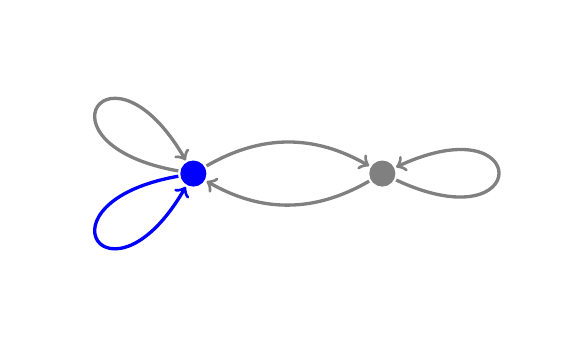
\begin{tikzpicture}[scale=0.8]
\node[circle, fill=blue, ultra thick] (In) at (0,0) {};
\node[circle, fill=gray, ultra thick] (Out) at (3,0) {};
\draw[->, very thick, gray] (In) to[bend left] (Out);
\draw[->, very thick, gray] (Out) to[bend left] (In);
\draw[->, very thick, gray] (In) to[loop left, in=120, out=170, looseness=30] (In);
\draw[->, very thick, blue] (In) to[loop left, in=-120, out=-170, looseness=30] (In);
\draw[->, very thick, gray] (Out) to[loop right, in=25, out=-25, looseness=30] (Out);
\end{tikzpicture}
\end{center}
我们可以定义从 \(G\) 到上面的有向图 \(\Omega\) 的映射,
将在 \(H\) 中的点射到蓝色的顶点, 不在的则射到灰色的顶点.
五种边也可以自然地映射到 \(\Omega\) 中的五条边. 那么可以发现
子图 \(H \hookrightarrow G\) 与映射 \(G \to \Omega\)
是一一对应的.

总结上面两个例子的共性, 我们可以定义\textbf{子对象分类器}的
概念. 如果一个对象 \(\Omega\) 满足任何 \(G\) 的子对象都可以
表示为 \(G \to \Omega\) 的态射, 就称这个对象为子对象分类器,
因为它分类了子对象中所有可能出现的情况.
我们来把这个定义严谨化. 什么是子对象呢? 首先需要注意的是,
\emph{子对象不是对象}. 子群不是群, 因为如果子群是群的话,
同构的群应该被视作完全相同. 然而 \(\mathbb Z\)
的两个子群 \(2\mathbb Z\) 与 \(3\mathbb Z\)
尽管同构, 但是显然不应该看作同一个子群. 子群 \(H \subseteq G\)
应当还包含它在群 \(G\) 中的哪个位置的信息. 因此, 我们
定义子群为一个群 \(H\) 配备一个单射 \(H \rightarrowtail G\).
在范畴中, 单射的定义是一个箭头 \(f : A \to B\), 满足
对于任何 \(u,v : C \to A\) 都有
\[f\circ u = f \circ v \implies u = v.\]
读者可以验证在集合范畴中这的确给出单射.

\begin{definition}
一个对象 \(\Omega\) 配备一个态射
\(t : \star \to \Omega\)
称为\textbf{子对象分类器}\footnote{我们不需要
对这个态射做任何要求, 但是可以可以证明如果子对象分类器存在,
那么 \(t\) 必然是单射, 换句话说 \(\star\) 是 \(\Omega\)
的子对象. 同时, \(\star\) 一定是终对象.}, 当且仅当对于任何单射
\(i : A \rightarrowtail X\), 都有唯一的映射
\([i] : X \to \Omega\) 与 \(\eta : A \to \star\)
使得以下图表是拉回.
\[\begin{tikzcd}
A && \star \\
\\
X && \Omega
\arrow["{[i]}", from=3-1, to=3-3]
\arrow["t"', from=1-3, to=3-3]
\arrow["i", tail, from=1-1, to=3-1]
\arrow["\eta", from=1-1, to=1-3]
\arrow["\lrcorner"{anchor=center, pos=0.125}, draw=none, from=1-1, to=3-3]
\end{tikzcd}\]
\([i]\) 被称为子对象的\textbf{特征映射}.
\end{definition}

在上面举例的图范畴中, \(\star\) 是一个点与一个自环
构成的图, \(\star \to \Omega\) 射到上图的蓝色子图.
请读者检查这确实符合定义. 如果读者有一些几何背景,
或许会觉得这个图非常熟悉.
\begin{definition}
给定一个拓扑群 \(G\), 定义其\textbf{分类空间}为
\(G\)-主丛 \(\pi : \mathrm{E}G \to \mathrm{B}G\),
使得对于任何 \(G\)-主丛 \(\gamma : A \to X\), 都有
唯一的映射 \(\tilde\gamma\) 与 \(\eta\), 使得以下
图表是拉回. \(\tilde\gamma\) 称为\textbf{分类映射}.
\[\begin{tikzcd}
A && \mathrm{E}G \\
\\
X && \mathrm{B}G
\arrow["{\tilde\gamma}", from=3-1, to=3-3]
\arrow["\pi"', from=1-3, to=3-3]
\arrow["\gamma", from=1-1, to=3-1]
\arrow["\eta", from=1-1, to=1-3]
\arrow["\lrcorner"{anchor=center, pos=0.125}, draw=none, from=1-1, to=3-3]
\end{tikzcd}\]
\end{definition}
分类空间是 \(G\)-主丛的分类器,
而子对象分类器是子对象的分类器.
这些定义的思想与模空间等也有联系.

尽管定义看起来很简短, 初等意象实际上包含了非常丰富的结构.
它实际上有所有的有限余极限, 并且是局部积闭的.
实际上, 如果初等意象有所有的余极限(还需要加上一些
防止罗素悖论的条件), 那么它就是Grothendieck意象.

\section{内语言}\label{category:inner}\berry{2}
\subsection{点集}
对于任何对象 \(A\), 从终对象出发的箭头集合 \(\hom(1,A)\)
称为 \(A\) 的\textbf{点集}. 如在集合范畴中这就是 \(A\)
的所有元素; 在拓扑空间范畴中, \(1\) 是单点拓扑空间,
\(\hom(1,A)\) 恰好就是拓扑上 \(A\) 的点集; 图的范畴
中, \(1\) 是有一个点与一个自环的图, 因此 \(\hom(1,A)\)
就是 \(A\) 上所有自环的集合.

可以看到, 从点集中可以探测到对象的一定信息, 但并不是全部
的信息. 在极端情况下, 点集完全不提供信息. 如在群范畴中,
终对象 \(1\) 是单元素群, 而 \(1 \to G\) 必然将其射到
单位元, 因此完全无法提供关于 \(G\) 的任何信息.\footnote{注意到
这样 \(1\) 也符合始对象的定义. 如果一个范畴中某个对象
既是始对象也是终对象, 那么我们称它为\textbf{零对象}.
交换代数中研究的许多范畴都有零对象.}

有没有什么办法用 \(\hom\) 集合探测更多信息呢? 我们
可以考虑不使用 \(1\), 而是使用一般的对象. 定义集合
\(\hom(U, A)\) 为 \(A\) 的 \(U\)\textbf{-状点集}. 在有向图
的范畴中, 如果我们取图 \(I = \boxed{\bullet \to \bullet}\),
那么图 \(G\) 的 \(I\)-状点集就是它的边的集合.
在代数几何中, 这样的广义点起了非常重要的作用.
方程 \(x^2 + y^2 = 1\) 定义了一个概形.
它的 \(\mathrm{Spec}(\mathbb Q)\)-状点集就是
有理点集 \(\{(x,y) \in \mathbb Q^2 \mid x^2 + y^2 = 1\}\),
\(\mathrm{Spec}(\mathbb F_p)\)-状点集就是模 \(p\)
意义下的解集, 等等. 我们前面定义的单射也可以用广义点
的语言重新表述: 一个态射 \(f : A \to B\) 是单射
当且仅当它诱导的所有广义点集的映射
\(\hom(U, A) \to \hom(U, B)\) 都是集合上的单射.

给定态射 \(f : U \to V\), 我们就能得到一个点集之间的函数
\(\hom(V, A) \to \hom(U, A)\), 即态射复合操作.
因此 \(\hom(-,A)\) 得到了一个函子
\(\mathcal C^{\cons{op}} \to \cons{Set}\).
这个函子组织了 \(A\) 的所有广义点集的信息.
那么这个办法能不能得到全部的信息呢? 令人惊讶的是,
答案是肯定的.

\begin{lemma}[米田]
\(\hom(-,A)\) 与 \(\hom(-,B)\) 之间的自然变换
与 \(A\) 到 \(B\) 的态射一一对应. 进一步说, 函子
\(\yo(A) = \hom(-,A)\) 是满忠实函子.
这里 \(\yo\) 是日文名“米田”的第一个音节.
\end{lemma}

我们可以给一个使用米田引理的例子. 如果某个范畴中有乘积
\(A \times (B \times C)\) 与 \((A \times B) \times C\),
它们是否同构呢? 如果直接使用泛性质, 证明会非常繁琐.
而使用米田引理, 这就化为简单的计算:
\[\begin{aligned}
\yo(A \times (B \times C))
&= \hom(-, A \times (B \times C))\\
(\text{泛性质})\quad &\cong \hom(-, A) \times (\hom(-, B) \times \hom(-, C))\\
(\text{集合的性质})\quad &\cong (\hom(-, A) \times \hom(-, B)) \times \hom(-, C)\\
(\text{泛性质})\quad &\cong \hom(-, (A \times B) \times C)\\
&= \yo((A \times B) \times C).
\end{aligned}\]
其中, 中间由于是集合的乘积, 显然是满足结合律的.
由此我们得到两个对象经过 \(\yo\) 之后是同构的.
但是由于这个函子是满忠实函子, 因此这两个对象本身也
必然同构.

米田引理告诉我们, 想要了解一个对象 \(A : \mathcal C\),
我们只需要了解 \(\yo(A) : \mathcal C^{\cons{op}} \to \cons{Set}\).
反过来想, 如果我们提供了一个函子 \(F : \mathcal C^{\cons{op}} \to \cons{Set}\),
它就可以视作\textbf{广义对象}. 这个思想与广义函数的定义
非常相似. 想要了解连续函数 \(f : [0,1] \to \mathbb R\),
我们只需要了解每个 \(\int_0^1 f(x)g(x)\,\mathrm dx\),
其中 \(g\) 是测试函数. 因此如果我们定义了一个线性泛函,
将测试函数映射到实数, 那么它就可以看作一种广义的函数.
这样, 原本的函数就是广义函数的子集, 并且我们得到了类似
\(\delta\)函数等新的对象.

\subsection{Kripke--Joyal翻译}

考虑一个态射 \(\varphi : X \to \Omega\), 这也
确定了一个子对象 \(\{x : X \mid \varphi(x)\}\).
\[\begin{tikzcd}
& {\{x \mid \varphi(x)\}} & 1 \\
1 & X & \Omega
\arrow[from=1-2, to=1-3]
\arrow["t", from=1-3, to=2-3]
\arrow["\chi_{\varphi}", from=1-2, to=2-2]
\arrow["\varphi"', from=2-2, to=2-3]
\arrow["p"', from=2-1, to=2-2]
\arrow["\tilde p", dashed, from=2-1, to=1-2]
\end{tikzcd}\]
如果有一个点 \(p : 1 \to X\) 满足存在
\(\tilde p : 1 \to \{x \mid \varphi(x)\}\)
使得上图交换, 那么就称点\(p\) \textbf{满足} \(\varphi\).%
\footnote{事实上, 这等价于说 \(\varphi \circ p = t\).
其等价性是很好的范畴论习题, 但是在没有子对象分类器时就
只能依靠原本的定义. 在广义点的情况下也有类似的等价.}
我们进一步考虑广义点集. 如果广义点 \(p : U \to X\) 存在
\(\tilde p : U \to \{x \mid \varphi(x)\}\) 使得
上图交换, 那么就称广义点\(p\) \textbf{满足} \(\varphi\).
这写作 \(p \vDash \varphi\), 如果箭头 \(p\) 没有歧义,
也会写作 \(U \vDash \varphi\).

我们以Zariski意象为例, 将这些定义展开, 看看会得到什么.
Zariski意象\(\cons{Zar}\)中, 其对象包含了所有的环.
对于任意环 \(R\):
\begin{center}
\begin{tabular}{c @{\(\color{gray}{}\iff{}\)} p{0.5\textwidth}}\hline
\(R \vDash \top\) & \(R\) 中 \(1 = 1\).\\
\(R \vDash \bot\) & \(R\) 中 \(0 = 1\).\\
\(R \vDash \phi\wedge\psi\) & \(R \vDash \phi\)
  且 \(R \vDash \psi\).\\
\(R \vDash \phi\vee\psi\) & \(R\) 中存在有限个元素
  \(\sum_i f_i = 1\), 使得对于每个 \(i\) 都有
  \(R[f_i^{-1}] \vDash \phi\) 或
  \(R[f_i^{-1}]\vDash \psi\).\\
\(R \vDash \phi\Rightarrow\psi\) & 对于任何 \(R\)-代数
  \(S\), 如果 \(S \vDash \phi\) 则 \(S \vDash \psi\).\\\hline
\end{tabular}
\end{center}
这覆盖了许多交换代数中常见的操作.
进一步研究这样的语言, 可以大大简化复杂对象的研究.
从另一个视角, 意象可以说是提供了一个“数学宇宙”. 在这个宇宙
中可以进行各种数学操作. 每个宇宙都有自己独特的性质.
读者可以参考~\cite{oliveri:2022:structure},
其中第四章是对这些数学宇宙的简明易懂的介绍.
关于Zariski意象在代数几何中的应用, 读者可以阅读~\cite{blechschmidt:2021:internal}.

Kripke--Joyal翻译仅仅为意象提供了内语言. 对于有其他结构
的范畴, 就有各自对应的内语言与翻译方式.

\subsection{ETCS}
排中律在内语言中的翻译为 \(\Omega = 1 + 1\), 即
子对象分类器是两个终对象的不交并. 在集合范畴中这是成立的,
但是在之前举例的图范畴中, 终对象是一个点上有一个自环,
但子对象分类器有两个点和五条边, 不是两个终对象的不交并.
许多意象的内语言中, 排中律是不成立的.\footnote{内语言中
排中律是否成立与外部语言是不一样的. 集合范畴中排中律成立,
等价于外部语言的排中律成立; 图范畴中无论如何排中律都
不成立; 相反地, 在有限集合构成的范畴中排中律无论如何都
成立.} 如定理~\ref{ch:diaconescu} 所述, 如果选择公理
成立, 排中律也成立.

% (...) 选择公理?

在范畴中, 一个态射不再由它在点集上的表现决定. 例如图范畴
中, 只知道一个态射在点集上的表现, 仍然无法决定边如何映射.
我们可以做一个定义.
\begin{definition}
我们称满足这个条件的范畴是\textbf{良点}的(well-pointed):
对于任何两个态射 \(f, g : X \to Y\),
如果它们诱导点集上的映射 \(\hom(1, X) \to \hom(1,Y)\)
相等, 则 \(f = g\).
\end{definition}
集合范畴与拓扑空间范畴都是良点的.

在本节开头提到的ETCS可以简洁地定义为(初等)意象上的三条公理:
良点性, 选择公理与无限公理. 无限公理在ZFC集合论中也有出现,
大致含义就是“自然数集合存在”. 我们至少需要这样一条公理, 否则
无法构造出任何无限大的对象. 在范畴论中, 自然数对象
(natural numbers object, 缩写为NNO)的定义与类型论
中自然数类型的定义很相似.
\begin{definition}
\textbf{自然数对象}是一个对象 \(\mathbb N\), 配备
了两个态射 \(1 \xrightarrow{\cons{z}} \mathbb N \xrightarrow{\cons{s}} \mathbb N\),
分别表示零与后继. 对于任何其他对象 \(A\) 配备两个态射
\(1 \xrightarrow z A \xrightarrow s A\), 都有
唯一的态射 \(u : \mathbb N \to A\) 使得以下图表交换.
\[\begin{tikzcd}[row sep=3]
& {\mathbb N} && {\mathbb N} \\
1 \\
& A && A
\arrow["z"', from=2-1, to=3-2]
\arrow["s"', from=3-2, to=3-4]
\arrow["{\cons{z}}", from=2-1, to=1-2]
\arrow["{\cons{s}}", from=1-2, to=1-4]
\arrow["u"{description}, from=1-2, to=3-2]
\arrow["u"{description}, from=1-4, to=3-4]
\end{tikzcd}\]
\end{definition}
满足ETCS公理的范畴, 表现得非常像集合范畴, 基本满足数学中
要求集合范畴满足的所有性质. 因此ETCS可以作为类似ZFC的集合论
使用.

\section{内语言与类型论}

(...)
